\section{Marco Teórico}

\subsection{Microcontrolador ATmega328P}
El ATmega328P es un MCU AVR de 8 bits con 32\,KB de memoria FLASH para programa, 2\,KB de SRAM y 1\,KB de EEPROM. Funciona típicamente a 16\,MHz y ofrece periféricos integrados: temporizadores, USART, SPI, I\textsuperscript{2}C (TWI), ADC de 10 bits e interrupciones internas y externas. Su arquitectura Harvard y las instrucciones sencillas permiten control en tiempo real con bajo consumo. 

\subsection{Registros de propósito general}
Dispone de 32 registros de 8 bits (R0–R31) de acceso rápido. Tres pares forman punteros de 16 bits: X (R27:R26), Y (R29:R28) y Z (R31:R30), útiles para direccionamiento indirecto y acceso a tablas. El uso disciplinado de estos registros (convención de qué se preserva y qué se clobbera) facilita escribir rutinas eficientes y evitar efectos laterales.

\subsection{Entradas y Salidas Digitales}
Cada pin puede configurarse como entrada o salida mediante los registros DDRx; el estado lógico se escribe en PORTx y se lee en PINx. Como entrada, puede habilitarse la resistencia \textit{pull-up} interna; como salida, el pin puede manejar LEDs, pulsadores y otros dispositivos a través de resistencias o etapas de potencia. Para pulsadores se recomienda tratamiento de rebotes; para LEDs, usar resistencias limitadoras y respetar las corrientes máximas del puerto. El mapeo de los puertos para el ATmega328P en plataforma Arduino se encuentra en el anexo \ref{anexo:Microcontrolador_ATmega328P}.


\subsection{Stack Pointer}
El stack pointer es una herramienta utilizada dentro de la programación del microcontrolador. El stack pointer es un puntero interno del microcontrolador (similar a X, Y o Z) el cual tiene una serie de operaciones asignadas, y un comportamiento específico. El stack pointer se inicializa al final de la memoria RAM, alejado de todo para intentar no molestar al resto. Véase anexo \ref{anexo:Stack_Pointer}.

Allí el stack pointer queda como la cima de la pila y, en AVR, la pila crece hacia direcciones más bajas: un PUSH decrementa primero el SP y luego escribe el dato; un POP lee el dato y después incrementa el SP. Las llamadas a subrutinas (CALL/RCALL) empujan automáticamente la dirección de retorno (PC) a la pila y RET la recupera. En una interrupción, el hardware apila el PC y el registro de estado SREG; RETI los restaura. Además, las rutinas suelen guardar con PUSH los registros que van a usar y devolverlos con POP al salir para no corromper el contexto.

Instrucciones como call, rcall, o las interrupciones dependen de la inicialización previa del Stack Pointer, para poder funcionar de manera adecuada, ya que el Stack Pointer es el que se encarga de guardar las direcciones de memoria a las cuales estas instrucciones deben retornar luego de terminar la ejecución, de no estar inicializado el Stack Pointer, el programa no sabría a donde volver luego de una interrupción, muy probablemente yendo a una dirección del programa aleatoria y rompiendo el flujo del codigo. Véase anexo 

\subsection{Delay activo}
Un delay activo es una pieza de código que toma en cuenta la velocidad de ejecución del microcontrolador, para ejecutar un número de instrucciones (inútiles) concreto, representando un pasaje de tiempo específico, para luego retornar al flujo del programa. Son fáciles de usar, pero no es recomendable abusar de ellas debido a ineficiencias energéticas, y que el programa se mantiene ocupado la mayor parte del tiempo en el temporizador, en lugar de poder dedicarse a hacer otras tareas. Véase anexo \ref{anexo:Delay_Activo}, allí se encuentra un ejemplo de un delay activo.

\subsection{Timers}
Timer 0 y 2 son de 8 bits. Timer 1 es de 16 bits, por lo que puede contar intervalos más largos y con mejor resolución. Cada timer toma su reloj de la CPU y lo divide con un prescaler \(N\) La ecuación para calcular el tiempo de desborde es:

\[
    \frac{(2^{k} - C_{\text{inicio}})\cdot \text{N}}{f_{\text{CPU}}} = t_{\text{deseado}}
\]


Esta ecuación determina el tiempo que le tomaría al contador hacer un desbordamiento (overflow) en base a la frecuencia a la cantidad de bits del contador (k), la frecuencia de trabajo del microcontrolador, el tiempo o conteo con el que se inicie el contador, y el prescaler con el que esté configurado. En el anexo \ref{anexo:Configuracion_Timer_1} podrá encontrar un procedimiento detallado de como configurar el Timer 1.

\subsection{Interrupciones externas}

    \begin{figure}[H]
    \centering
    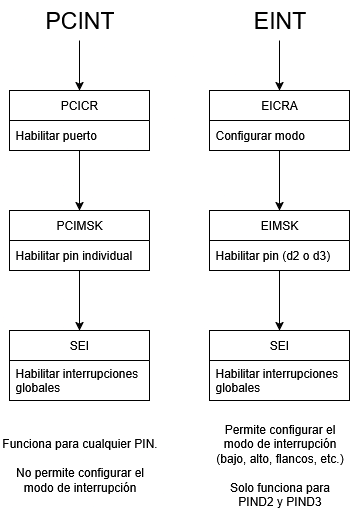
\includegraphics[width=0.7\linewidth]{./Anexos/Marco Teorico/External Interrupts/Interrupt diagram.png}
    \caption{Flujo de configuración de interrupciones externas. Fuente: Elaboración propia.}
    \label{fig:InterruptDiagram}
    \end{figure}

    Ver anexo \ref{anexo:Interrupciones_Externas} para información detallada de como configurar estas interrupciones.

    \subsubsection{EINT}
    Interrupciones externas en INT0 e INT1 (pines PD2 y PD3). Permiten elegir el tipo de disparo: nivel bajo, cambio lógico, flanco de bajada o de subida. Se configuran en EICRA y se habilitan en EIMSK; las rutinas de servicio son INT0\_vect e INT1\_vect.

    \subsubsection{PCINT}
    Interrupción por cambio de pin. Detecta cualquier cambio en pines habilitados de los puertos B, C y D (grupos PCINT0\_7, PCINT8\_14, PCINT16\_23). No distingue flancos, pero funciona en casi todos los pines. Se habilita por grupo con PCICR y por pin con PCMSKx; las rutinas son PCINT0-vect, PCINT1-vect y PCINT2-vect.

\subsection{SRAM}

Usando \texttt{.dseg} se puede reservar espacio en SRAM. Luego, con \texttt{lds}/\texttt{sts} se lee o escribe esa variable. También pueden usarse punteros X, Y o Z para recorrer posiciones contiguas (como un arreglo). Ver anexo \ref{anexo:SRAM}.

Nota: Existen 2kb de memoria RAM, el stack pointer vive dentro de la RAM así que uno debe ser precavido con el uso excesivo de este recurso, si se desea guardar gran cantidad de valores estáticos, una mejor alternativa podrá ser la memoria FLASH.

\subsection{FLASH}

Utilizando .cseg y una dirección segura como 0x300 para guardar datos, se puede utilizar la misma memoria FLASH para guardar datos constantes como LUTs, fotogramas, cadenas de texto, etc. Estos datos no pueden ser modificados, pero existen 32kb de espacio en memoria FLASH para guardar información, por lo que es menos limitante que la SRAM (2kb).

Para acceder a datos guardados en program memoria del programa (FLASH) se puede hacer haciendo uso del puntero Z y la instrucción \texttt{lpm}. En ``Z'' Se carga la dirección a Z cargando las partes bajas y altas de la dirección a ZL y ZH respectivamente. En los AVR  ``clásicos'' (como el ATmega328P), las etiquetas en memoria de programa (\texttt{.cseg}) están en direcciones de palabra (cada instrucción ocupa 16 bits), pero la instrucción LPM usa una dirección en bytes en el registro Z. Por eso se hace $<$$<$ 1 (multiplicar por 2): convierte la dirección en palabras de la etiqueta a dirección en bytes para LPM. Y \texttt{Z+} indica que luego de realizar \texttt{lpm}, se incremente en 1 el puntero Z. Véase anexo \ref{anexo:FLASH}.

\subsection{Bit masks}
Una máscara es un número binario, pero en una máscara lo que nos importa es la posición de los unos y ceros en lugar del valor mismo que representan. Un mismo valor binario puede representar un número o una máscara, solo depende de como lo mires.  

\texttt{ldi r16, 0b00001010 out PORTB, r16} carga una máscara de bits al puerto B para encender los pines 1 y 3, y apagar el resto, pero también se puede ver como que se está cargado el número 10 al puerto B (\texttt{ldi r16, 10 out PORTB, r16})

Saber operar con máscaras se vuelve útil cuando, por ejemplo, se busca afectar solo uno o varios bits en específico de un registro. En ese caso,  Lo que se hace primero es leer el registro, luego se realizar una operación lógica con la máscara que representa los bits que se quieren afectar, y por último se carga la máscara modificada al registro. Este tipo de operaciones se vuelve muy común cuando se trabajan con matrices LED, donde es muy común tener que mezclar puertos entre filas y columnas. Véase anexo \ref{anexo:Bit_Masks}.


\subsection{LUT}
Para trabajar de manera ordenada en el desorden. Convierte al dolor de cabeza que son los puertos, en simples operaciones de lectura de FLASH, y modificación de punteros. Véase anexo \ref{anexo:Look_Up_Table}

\begin{figure}[H]
  \centering
  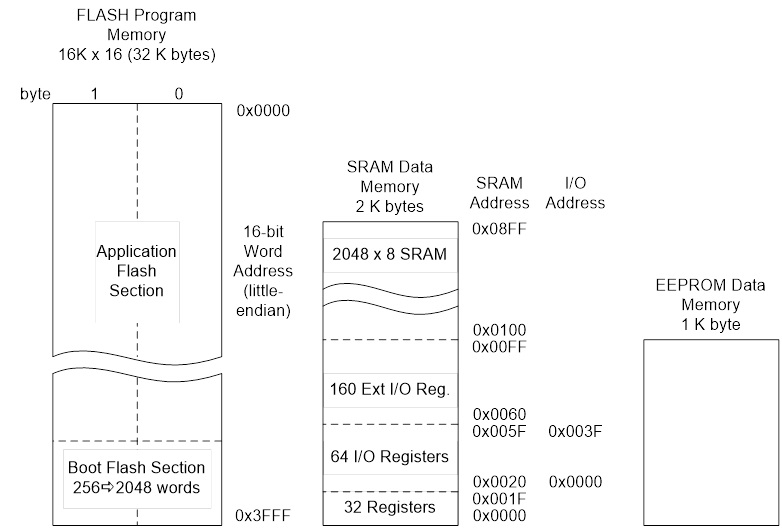
\includegraphics[width=\linewidth]{./Anexos/Memory Map.jpg}
  \caption{Mapa de memoria y espacios de direcciones en AVR de 8 bits. Fuente: \cite{arxterra_avr_addressing_modes}.}
  \label{fig:avr-memory-map}
\end{figure}

\subsection{USART asíncrono}
La USART en modo asíncrono permite comunicación serie full-dúplex con tramas que incluyen un bit de inicio, 8 bits de datos (habitual), paridad opcional y 1–2 bits de parada. En el ATmega328P las líneas son RXD (PD0) y TXD (PD1).

La velocidad se ajusta con el registro UBRR a partir de la frecuencia de la CPU y el baud rate deseado. En modo normal (U2X0=0) se usa el reloj dividido por 16; en modo doble velocidad (U2X0=1) se usa el reloj dividido por 8, lo que mejora la precisión a ciertos baudios.

La configuración básica habilita recepción y transmisión en UCSR0B, define formato de trama en UCSR0C y consulta estados en UCSR0A; el registro de datos es UDR0. Más detalles y ejemplos en el anexo \ref{anexo:USART_Asincrono}.



\subsection{Ring Buffer}
Un ring buffer es una cola circular que usa dos índices: \textit{head} para escribir y \textit{tail} para leer. Al llegar al final del arreglo, ambos vuelven al inicio (se “enroscan”), por eso es circular. La cola está vacía cuando \textit{head} y \textit{tail} son iguales; está llena cuando avanzar \textit{head} una posición alcanzaría a \textit{tail}. Elegir un tamaño potencia de dos simplifica el avance de índices (se puede usar una máscara en lugar de un módulo). En USART suele emplearse para recibir y transmitir sin bloquear: la ISR coloca bytes en la cola y el código principal los consume. Conviene proteger la actualización de índices compartidos y decidir qué hacer si se llena la cola. Más detalles en el anexo \ref{anexo:Ring_Buffer}.



\subsection{USART asíncrono con Ring Buffer}
La combinación de USART asíncrono con un ring buffer permite comunicación serie sin bloqueo. En recepción, la ISR de RX lee \texttt{UDR0} y encola el byte en el buffer de entrada; la aplicación lo desencola cuando conviene. En transmisión, la aplicación encola datos en el buffer de salida y habilita la interrupción \textit{Data Register Empty}; la ISR va sacando bytes y cargándolos en \texttt{UDR0}, deshabilitando la interrupción cuando la cola queda vacía. Esta arquitectura evita esperas activas y minimiza la pérdida de datos bajo carga. Es recomendable usar tamaños potencia de dos, proteger la actualización de índices compartidos y definir una política ante desbordes (descartar lo nuevo o lo viejo, o espera activa). Detalles y esquema de inicialización en el anexo \ref{anexo:USART_Asincrono_con_Ring_Buffer}.


\subsection{Automatización y Máquinas de Estado}
Una máquina de estados modela el proceso como un conjunto finito de estados (p.\,ej., espera, mover cinta, punzonar, retroceso) y transiciones disparadas por eventos (sensores, temporizadores, comandos por USART). En cada estado se definen acciones de entrada/salida (activar motores, habilitar solenoide, actualizar LEDs) y las condiciones para cambiar al siguiente estado. Este enfoque hace el control \textit{determinista}, facilita el manejo de errores y simplifica la verificación de seguridad (interlocks, límites de carrera, anti-rebote en pulsadores). En el ATmega328P se implementa de forma directa con un “switch” sobre la variable de estado y saltos condicionales, manteniendo la lógica de transición en una sección única y clara. Los temporizadores e interrupciones proveen eventos periódicos y asincrónicos sin bloquear el ciclo principal. Un diagrama y la especificación de estados/transiciones se incluyen en el anexo \ref{anexo:Maquina_de_Estados}.


\subsection{Conversión Digital-Analógica (DAC R-2R)}
Un DAC (Digital to Analog Converter) es un dispositivo o técnica que permite transformar valores digitales (códigos binarios) en señales analógicas (tensiones o corrientes continuas y variables en el tiempo). Su importancia radica en que la mayoría de los sistemas electrónicos trabajan de manera digital, pero el mundo físico es analógico: audio, imágenes, señales de control de motores, etc.

El arreglo R-2R es una red de resistencias que se usa mucho para construir DACs simples y económicos. Se compone unicamente de dos valores de resistencias: una de valor R y otra de valor 2R, que se repiten en forma de escalera.

Cada bit del número digital controla un pin de los puertos del microcontrolador que conecta la red a una referencia de tensión (Vref) o a tierra. Gracias a la proporción entre Ry 2R, la red genera tensiones que corresponden al valor binario aplicado.

Una Look-up Table (LUT) es básicamente una tabla de valores precargada en la memoria que representa una señal digitalizada (por ejemplo, una onda seno). En lugar de calcular cada valor de la función en tiempo real, el microcontrolador ``lee'' la tabla en orden y envía los valores a un puerto configurado con un DAC. Cuando esos valores se aplican de manera periódica y con la velocidad adecuada, en la salida se reconstruye una señal analógica periódica.
    

\subsection{Matriz de LEDs}
Modelo 1088AS: matriz 8×8 de cátodo/anodo multiplexado, apta para control por filas y columnas. La disposición exacta de pines se encuentra en el anexo \ref{anexo:Matriz_de_LEDs_1088AS}. Para encender un LED específico, se aplica nivel 0 a la fila correspondiente y nivel 1 a la columna correspondiente.


\subsection{Plotter y Control de Movimiento}
Un plotter es un sistema de trazado que posiciona un útil (lápiz/solenoide) en X–Y para dibujar o marcar piezas. En ingeniería se usa para prototipado, plantillas y pruebas de control de movimiento.

El movimiento puede lograrse con motores paso a paso o con motores conmutados mediante relés/MOSFETs. En el primer caso se controlan pasos y dirección; en el segundo, sentido y velocidad (opcionalmente con PWM). El útil sube y baja con un solenoide controlado también por una salida digital.

Este plotter ya tiene un Arduino conectado al \texttt{PORTD}. Cada bit de \texttt{PORTD} activa una acción: arriba, abajo, izquierda, derecha, subir solenoide, bajar solenoide. La tabla de comandos está en el anexo \ref{anexo:Comandos_Plotter}.


\subsection{Macros}
En ensamblador, una macro es una plantilla de texto que el ensamblador expande en tiempo de ensamblado. No es una subrutina: no hay llamadas ni RET; el código se copia inline cada vez que se usa. Sirven para evitar repetir secuencias, parametrizarlas y hacer el código más legible. Véase anexo \ref{anexo:Macros}.

Entre las ventajas están la reutilización de patrones, la reducción de errores por copia y pega, y la posibilidad de recibir parámetros (puerto, bit, conteo, etc.), lo que permite adaptar la misma secuencia a distintos casos.

Como cuidado, cada expansión aumenta el tamaño del binario. Además, como el cuerpo se inserta tal cual, conviene documentar qué registros modifica (clobbers) y usar etiquetas locales para evitar choques de nombres.



